A seguir são apresentados os resultados obtidos ao executar a Rede Colorida de Petri utilizando a ferramenta CPN IDE.

\subsection{Estado inicial}

A Figura~\ref{fig:initial_state} representa a rede em sua condição inicial.
Todos os semáforos na rede encontram-se no estado fechado, indicado pela cor vermelha.

Nesse estágio, todas as transições responsáveis por mover fichas dos lugares vermelhos para os lugares verdes estão habilitadas.
Isso ocorre porque todos os lugares vermelhos possuem fichas em quantidade suficiente para ativar qualquer transição.
Cada um dos lugares vermelhos contém 2 fichas, possibilitando assim o disparo de qualquer transição de maneira arbitrária.

\begin{figure}[ht]
	\centering
	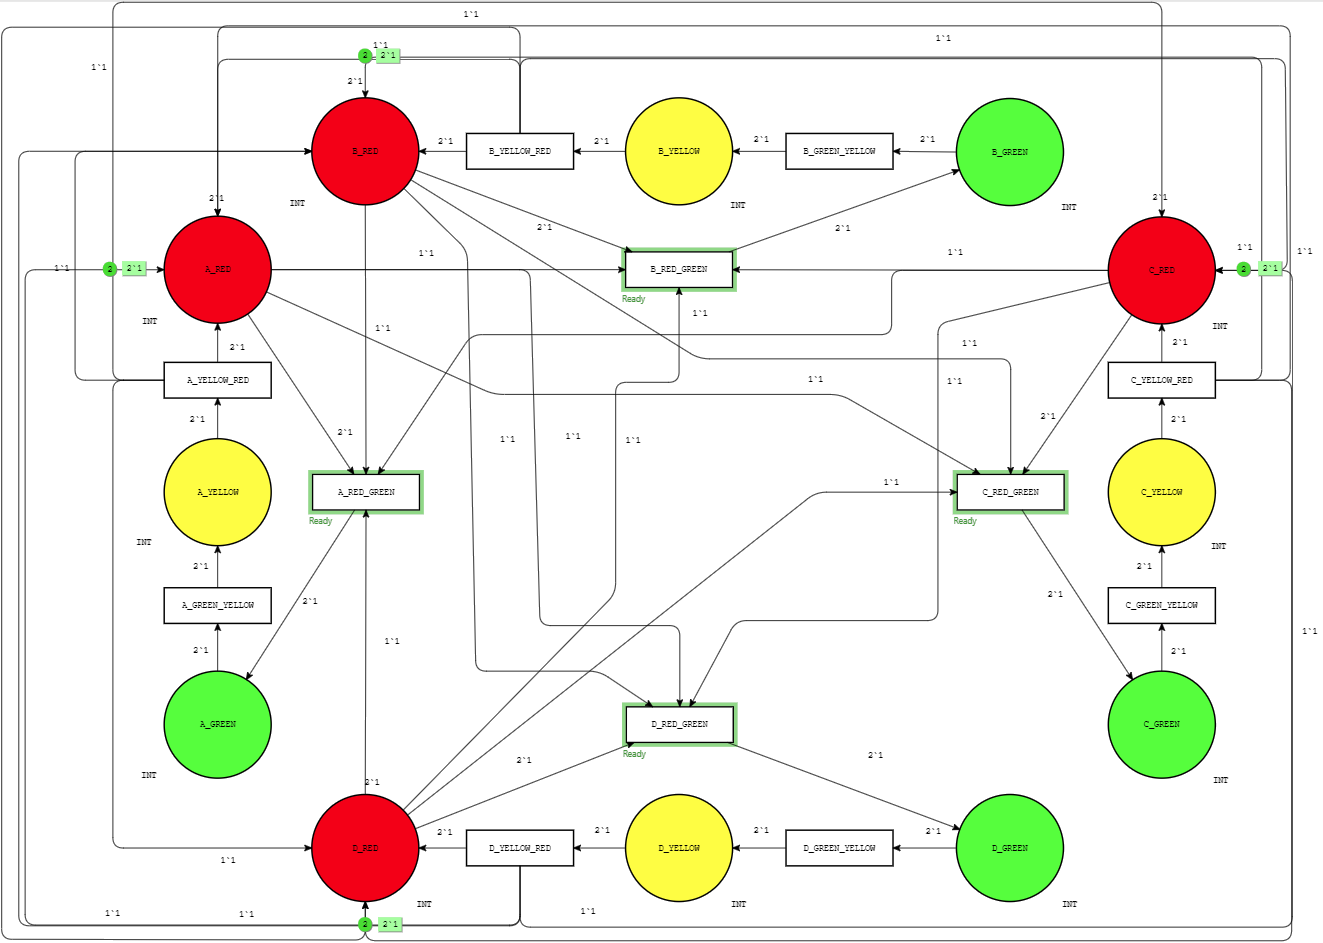
\includegraphics[width=1\textwidth]{images/initial_state.png}
	\caption{Estado inicial da rede}
    \label{fig:initial_state}
\end{figure}

\subsection{Disparo de uma transição em um semáfaro}

A Figura~\ref{fig:a_red_green_fired} representa a rede após o disparo de uma transição em um dos semáforos.
Neste caso, o semáforo A foi escolhido para ser acionado.
O semáforo A encontra-se no estado aberto, representado pela cor verde, enquanto os demais semáforos na rede permanecem no estado fechado.

Nesse estágio, apenas a transição responsável por mover uma ficha do lugar verde para o lugar amarelo do semáforo A está ativa.
Todas as outras transições nos outros semáforos estão desabilitadas, uma vez que não há fichas em quantidade suficiente para ativar essas transições.

\begin{figure}[ht]
	\centering
	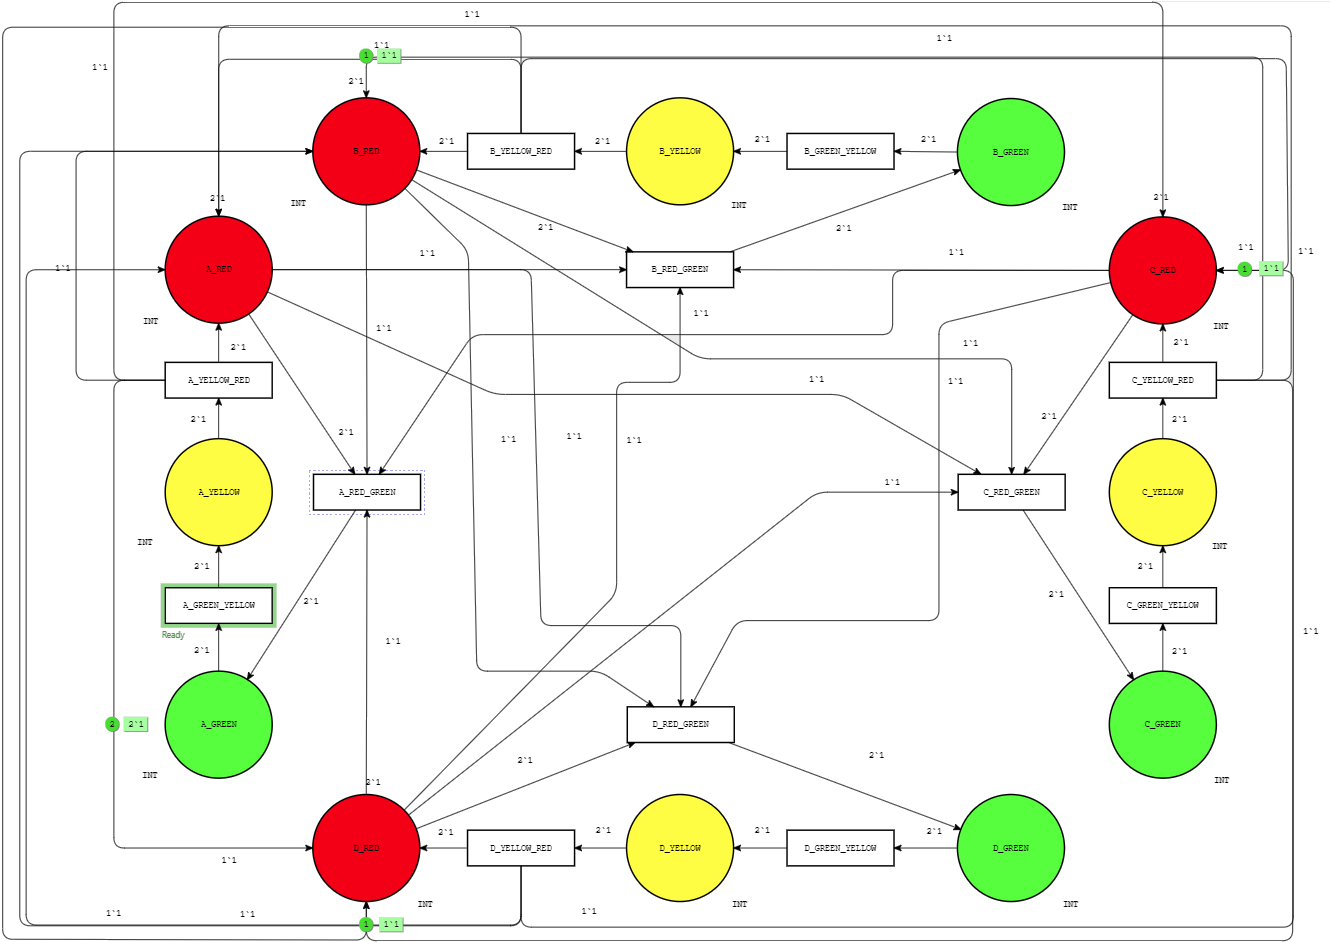
\includegraphics[width=1\textwidth]{images/a_red_green_fired.png}
	\caption{Transição do semáfaro A disparada}
    \label{fig:a_red_green_fired}
\end{figure}


\subsection{Restituição das fichas dos semáforos}

A Figura~\ref{fig:a_yellow_red_fired} representa a restituição das fichas aos semáforos correspondentes após a ativação da transição que altera a ficha do semáforo A do lugar amarelo para o lugar vermelho.
O disparo da transição que move a ficha do semáforo A do lugar verde para o lugar amarelo foi omitida.

Neste momento, o semáforo A está alterando seu estado para fechado, enquanto os demais semáforos na rede permanecem no estado fechado.
O disparo da transição que move uma ficha do lugar amarelo para o lugar vermelho do semáforo A está restituindo as fichas que foram retiradas dos outros semáforos.
Ela adiciona uma nova ficha em cada lugar vermelho de todos os semáforos.

Após essa restituição, todos os lugares vermelhos terão 2 fichas cada, possibilitando a mudança de estado de qualquer um dos quatro semáforos novamente, retornando a rede ao estado inicial.

\begin{figure}[ht]
	\centering
	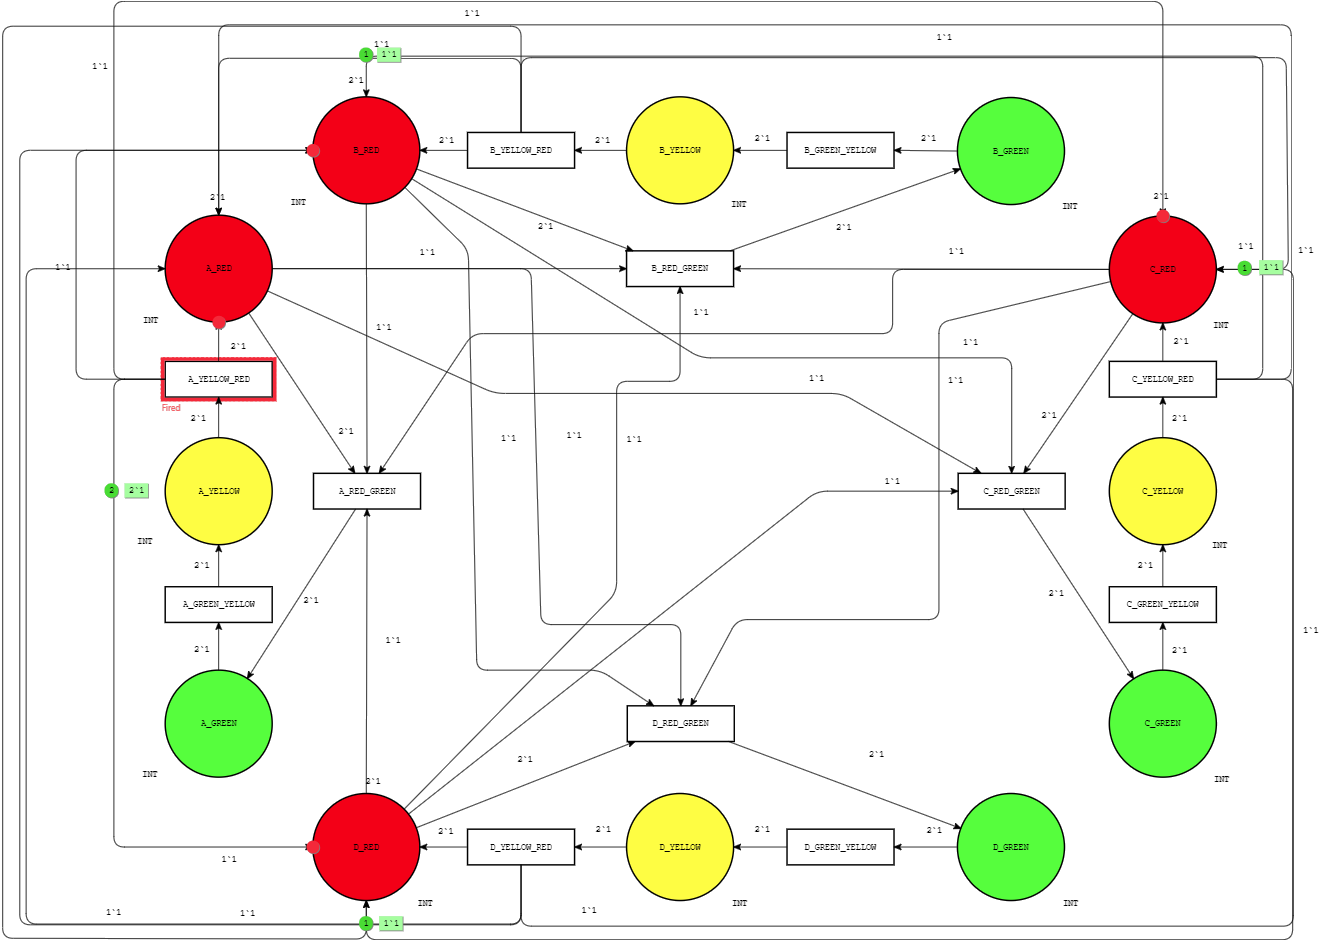
\includegraphics[width=1\textwidth]{images/a_yellow_red_fired.png}
	\caption{Restituição das fichas dos semáforos}
    \label{fig:a_yellow_red_fired}
\end{figure}

\clearpage